\title{The JPEG standard (ISO/IEC 10918-1)}

\maketitle
\tableofcontents

\section{Intro}
\begin{itemize}
\item JPEG = Joint Photographic Experts Group.
\item Developed in 1992 by the ISO \cite{CCITT.T81}.
\item True color (up to 24 bits/pixel) and grayscale (up to 8
  bits/pixel) images.
\item Eligible compression quality between $0-100$ \cite{Wallace91}.
\item Visually lossless reconstructions of color images for
  compression ratios about $1$ bits/pixel (bpp).
\item Based on the Discrete Cosine Transform (DCT).
\item Several working modes: lossy, lossless and hierarchical.
\end{itemize}

\section{Lossless JPEG \cite{JPEG-LS}}
\label{sec:LS-JPEG}
\begin{itemize}
\item Lossless.
\item Based on an spatial predictor and a 0-order static
  variable-length encoder (Huffman).
\item The block diagram is
  \begin{center}
    %\texfigure{0.8\textwidth}{!}{LS-JPEG_codec}
    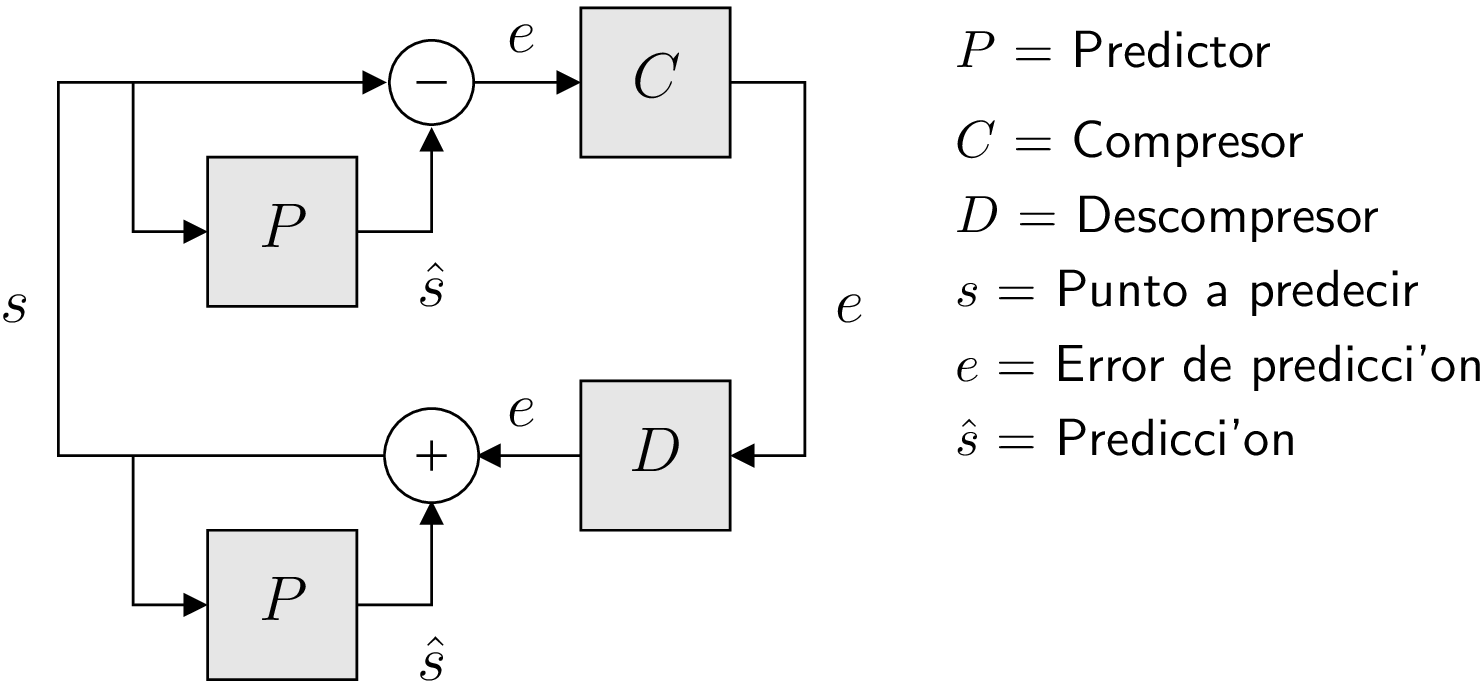
\includegraphics[width=0.8\textwidth]{LS-JPEG_codec}
  \end{center}
  where
  \begin{center}
    \begin{tabular}{c}
      Prediction Context \\
      %\texfigure{!}{!}{contexto_prediccion_JPEG}
      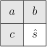
\includegraphics[width=2cm]{contexto_prediccion_JPEG}
    \end{tabular}
    \vspace{3ex}
    \begin{tabular}{|r|l|}
      \multicolumn{2}{c}{Predictors}\\
      \hline
      $P_0$ & $\hat{s}\leftarrow 0$\\
      $P_1$ & $\hat{s}\leftarrow a$\\
      $P_2$ & $\hat{s}\leftarrow b$\\
      $P_3$ & $\hat{s}\leftarrow c$\\
      $P_4$ & $\hat{s}\leftarrow a+b-c$\\
      $P_5$ & $\hat{s}\leftarrow a+(b-c)/2$\\
      $P_6$ & $\hat{s}\leftarrow b+(a-c)/2$\\
      $P_7$ & $\hat{s}\leftarrow (b+c)/2$\\
      \hline
    \end{tabular}
  \end{center}
\end{itemize}

\section{Codec LS-JPEG}
\subsection{Compressor}
\begin{enumerate}
\item Generate $\hat{s}$.
\item Compute the prediction error $e\leftarrow s - \hat{s}$.
\item Encode $e$.
\end{enumerate}
    
\subsection{Descompressor}
\begin{enumerate}
\item Generate $\hat{s}$ (idential to the Step 1 of the compressor).
\item Descode $e$.
\item Compute the pixel value $s\leftarrow e+\hat{s}$.
\end{enumerate}

\section{Huffman encoding in LS-JPEG}
\label{sec:compresion_huffman_LS-JPEG}
\begin{enumerate}
\item Search $e$ in $DIFF$ and select $SSSS$.
\item Encode $SSSS$ following the base code.
\item If $e>0$, then:
  \begin{enumerate}
  \item Encode $e$ using a binary number of $SSSS$ bits. The most
    significant bit of $e$ will be always 1.
  \end{enumerate}
\item Else:
  \begin{enumerate}
  \item Encode $e-1$ using a binary number of $SSSS$ bits. The most
    significant bit of $e$ will be always a 0.
  \end{enumerate}
\end{enumerate}

\section*{Example ($e=5$)}
\begin{itemize}
\item [1] $SSSS=3$.
\item [2] Output $\leftarrow 100_2$.
\item [3.a] Output $\leftarrow 101_2$.
\end{itemize}

\section*{Example ($e=-9$)}
\begin{itemize}
\item [1] $SSSS=4$.
\item [2] Output $\leftarrow 101_2$.
\item [4.a] Output $\leftarrow 0110_2$ (the four least significant
  bits of the two's complement of $-10_{10}$).
\end{itemize}

\newcommand{\categorias}{
  \begin{tabular}{|r|c|}
    \hline
    $SSSS$ & $DIFF$ \\
    \hline
    0 &                       0 \\
    1 &                     -1,1 \\
    2 &                  -3,-2,2,3 \\
    3 &         -7,$\cdots$,-4,4,$\cdots$,7 \\
    4 &        -15,$\cdots$,-8,8,$\cdots$,15 \\
    5 &       -31,$\cdots$,-16,16,$\cdots$,31 \\
    6 &       -63,$\cdots$,-32,32,$\cdots$,63 \\
    7 &      -127,$\cdots$,-64,64,$\cdots$,127 \\
    8 &     -255,$\cdots$,-128,128,$\cdots$,255 \\
    9 &     -511,$\cdots$,-256,256,$\cdots$,511 \\
    10 &    -1023,$\cdots$,-512,512,$\cdots$,1023 \\
    11 &   -2047,$\cdots$,-1024,1024,$\cdots$,2043 \\
    12 &   -4095,$\cdots$,-2048,2048,$\cdots$,4095 \\
    13 &   -8191,$\cdots$,-4096,4096,$\cdots$,8191 \\
    14 &  -16383,$\cdots$,-8192,8192,$\cdots$,16383 \\
    15 & -32767,$\cdots$,-16384,16384,$\cdots$,32767 \\
    16 &                    -32768 \\
    \hline
  \end{tabular}
}

%\newcommand{\codigos}{
%  \begin{tabular}{|r|r|l|}
%    \hline
%    $SSSS$ & Longitud  & C'odigo base \\
%    \hline
%    0 &  3 & 00 \\
%    1 &  4 & 010 \\
%    2 &  5 & 011 \\
%    3 &  5 & 100 \\
%    4 &  7 & 101 \\
%    5 &  8 & 110 \\
%    6 &  10 & 1110 \\
%    7 &  5 & 11110 \\
%    8 &  6 & 111110 \\
%    9 &  7 & 1111110 \\
%    10 &  8 & 11111110 \\
%    11 &  9 & 111111110 \\
%    12 & 10 & 1111111110 \\
%    13 & 11 & 11111111110 \\
%    14 & 12 & 111111111110 \\
%    15 & - & 1111111111110 \\
%    16 & - & 11111111111110 \\
%    \hline
%  \end{tabular}
%}

\newcommand{\codigos}{
  \begin{tabular}{|r|r|l|}
    \hline
    $SSSS$ & Base code \\
    \hline
    0 & 00 \\
    1 & 010 \\
    2 & 011 \\
    3 & 100 \\
    4 & 101 \\
    5 & 110 \\
    6 & 1110 \\
    7 & 11110 \\
    8 & 111110 \\
    9 & 1111110 \\
    10 & 11111110 \\
    11 & 111111110 \\
    12 & 1111111110 \\
    13 & 11111111110 \\
    14 & 111111111110 \\
    15 & 1111111111110 \\
    16 & 11111111111110 \\
    \hline
  \end{tabular}
}

\noindent\resizebox{1.0\textwidth}{!}{
  \begin{tabular}{cc}
    Category & Huffman code \\
    \categorias & \codigos
  \end{tabular}
}

\section{Huffman decoding in LS-JPEG}
\begin{enumerate}
\item Decode the $SSSS$ category using the base code.
\item Decode the magnitude. Let $x\leftarrow$ the next input bit.
\item If $x\ne 0$, then:
  \begin{enumerate}
  \item $e\leftarrow x << (SSSS-1) + \text{siguientes} (SSSS-1)$ bits.
  \end{enumerate}
\item Else:
  \begin{enumerate}
  \item $e\leftarrow (-1)~\text{AND}~(x << (SSSS-1)+\text{siguientes}~(SSSS-1)~\text{bits}+1)$.
  \end{enumerate}
\end{enumerate}

\section*{Example (decode $100101$)}  
\begin{itemize}
\item [1] $SSSS\leftarrow 3$.
\item [2] $x\leftarrow 1$.
\item [3.a] $e\leftarrow 2^2+$ next two input bits (01) $=101_2=5_{10}$.
\end{itemize}

\section*{Example (decode $1010110$)}
\begin{itemize}
\item [1] $SSSS\leftarrow 4$.
\item [2] $x\leftarrow 0$.
\item [4.a] (Using 8 bits of precision) $e\leftarrow$ $11111111_2$ AND
  ($0000_2+110_2+1_2) = 11110111_2 = -9_{10}$ (the four least
  significant bits of $0111_2$ are supposed to be $1$.
\end{itemize}

\section*{Lab}
\begin{enumerate}
\item Download \url{ftp.cs.cornell.edu:/pub/multimed/ljpg.tar.Z} and
  compile it.
\item Fill the table
\begin{verbatim}
  Codec | lena boats pepers zelda Average
--------+--------------------------------
      : |    :     :      :     :       :
ls-jpeg | ....  ....   ....  ....    ....
\end{verbatim}
\end{enumerate}

\section{Lossy JPEG}
\noindent Para una imagen RGB, el algoritmo básico consiste en:
\begin{enumerate}
\item Convertir la imagen al dominio YCbCr.
\item Submuestrear la crominancia.
\item Desplazar cada componente al rango $[-128,127]$.
\item Para cada componente (Y, Cb y Cr):
  \begin{enumerate}
  \item Aplicar la ($8\times 8$)-DCT a cada componente.
  \item Cuantificar los coeficientes DCT.
  \item Codificar entrópicamente los coeficientes cuantificados.
  \end{enumerate}
\end{enumerate}

\section{$[0,255]\rightarrow [-128,127]$}
\begin{itemize}
\item Every component should be 0-average. For this reason, if the
  values of the Y, Cb and CR components are in the range $[0,255]$,
  the $128$ is substracted (pixel-to-pixel) from each of them.
\item This is neccesary to reduce the arithmetic precision of the
  computation of the next step (the DCT).
\end{itemize}

\section{8x8 2D-DCT}
\begin{itemize}
\item Every component is
  \href{http://www.ual.es/~vruiz/docencia/JPEG/index.html#x1-160008}{DCT-transformed}
  in blocks of $8\times 8$ pixels.
\end{itemize}

\section{Basis functions of the 8x8 2D-DCT}
\begin{itemize}
\item Every $8\times 8$-DCT coefficient represent the weight that the
  corresponding pattern has to reconstruct the block.
\end{itemize}
\vspace{-3ex}
\begin{center}
  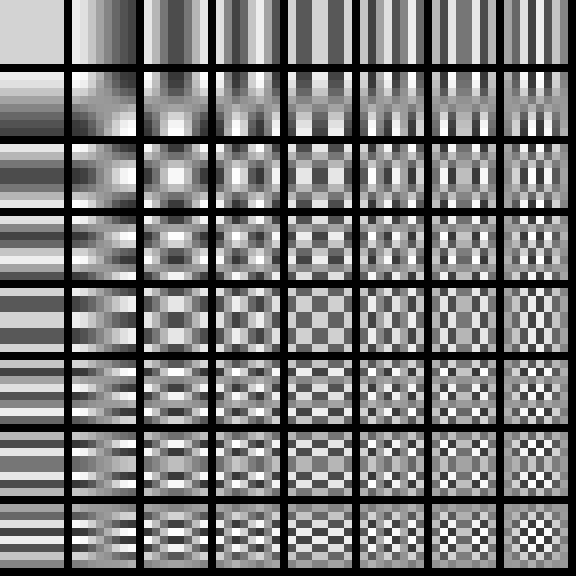
\includegraphics[height=0.75\textheight]{8x8_DCT_basis}
\end{center}

\section{Advantages of the 8x8 2D-DCT}
\begin{itemize}
\item \textbf{A lower total computational cost:}\\ It's faster the
  computation of $(\frac{N}{8}\times \frac{N}{8})$ $8\times 8$-DCTs
  than only one $N\times N$-DCT.
%  Es más rápido calcular
%  $(\frac{N}{8}\times \frac{N}{8})$ 2D-DCT's de $8\times 8$ puntos que
%  una 2D-DCT de $N\times N$ puntos ya que incluso la complejidad del
%  algoritmo rápido es superior a la lineal (${\mathcal O}(N)$ versus
%  ${\mathcal O}(N\log_2 N)$).
\item \textbf{``In-line'' operation:}\\
  The compressor process the images using blocks of $8\times 8$
  pixels, independiently of the size of the image.
\end{itemize}

\section{Scalar quantization}
\begin{itemize}
\item The main objective of the $8\times 8$-DCT is the spatial
  compactation of the energy in the image. As a consequence, a small
  set of coefficients accumulate the most part of this energy.
\item After this decorrelating step, the DCT coeffients are also very
  decorrelated. Therefore, scalar quantization is a good choice to
  quantize the spectral domain in order to reduce de amoun of encoded
  data.
\item The quantization generates a big number of DCT coefficients very
  close or equal to 0, following a Laplace probability distribution.
\newpage
\item The quantization step is so important in the result that the
  JPEG studied and determined the best quantization matrixes (one for
  the luma and other for the chroma).
\end{itemize}
  \begin{center}
    \resizebox{1\textwidth}{!}{
      \begin{tabular}{cc}
        Luminance & Chrominance \\
        \begin{tabular}{|rrrrrrrr|}
          \hline
          16 & 11 & 10 & 16 & 24 & 40 & 51 & 61 \\
          12 & 12 & 14 & 19 & 26 & 58 & 60 & 55 \\
          14 & 13 & 16 & 24 & 40 & 57 & 69 & 56 \\
          14 & 17 & 22 & 29 & 51 & 87 & 80 & 62 \\
          18 & 22 & 37 & 56 & 68 & 109 & 103 & 77 \\
          24 & 35 & 55 & 64 & 81 & 104 & 113 & 92 \\
          49 & 64 & 78 & 87 & 103 & 121 & 120 & 101 \\
          72 & 92 & 95 & 98 & 112 & 100 & 103 & 99 \\
          \hline
        \end{tabular}
        &
        \begin{tabular}{|rrrrrrrr|}
          \hline
          17 & 18 & 24 & 47 & 99 & 99 & 99 & 99\\
          18 & 21 & 26 & 66 & 99 & 99 & 99 & 99\\
          24 & 26 & 56 & 99 & 99 & 99 & 99 & 99\\
          47 & 66 & 99 & 99 & 99 & 99 & 99 & 99\\
          99 & 99 & 99 & 99 & 99 & 99 & 99 & 99\\
          99 & 99 & 99 & 99 & 99 & 99 & 99 & 99\\
          99 & 99 & 99 & 99 & 99 & 99 & 99 & 99\\
          99 & 99 & 99 & 99 & 99 & 99 & 99 & 99\\
          \hline
        \end{tabular}
      \end{tabular}
    }
  \end{center}
\begin{itemize}
\item At it can be seen, there is an overall tendence to preserve the
  low frequencies of the image.

\newpage

\item The quantization is described by
  \begin{equation}
    \text{2D-DCT}'[u,v] = \text{round}\Big(\frac{8\times 8\text{-DCT}[u,v]}{\text{Z}[u,v]}\Big)
  \end{equation}
  where $\text{Z}[\cdot,\cdot]$ is the quantization matrix.
\item It is possible to use different quantization matrixes, but they
  should be sent to the decompressor.
\end{itemize}

\section{Entropy encoding}
\begin{enumerate}
\item Substract to the DC coefficient the DC coefficient of the last
  encoded block. This calculus exploits the correlation between
  blocks.
\item Run the coefficients using the zig-zag pattern:
  \begin{center}
    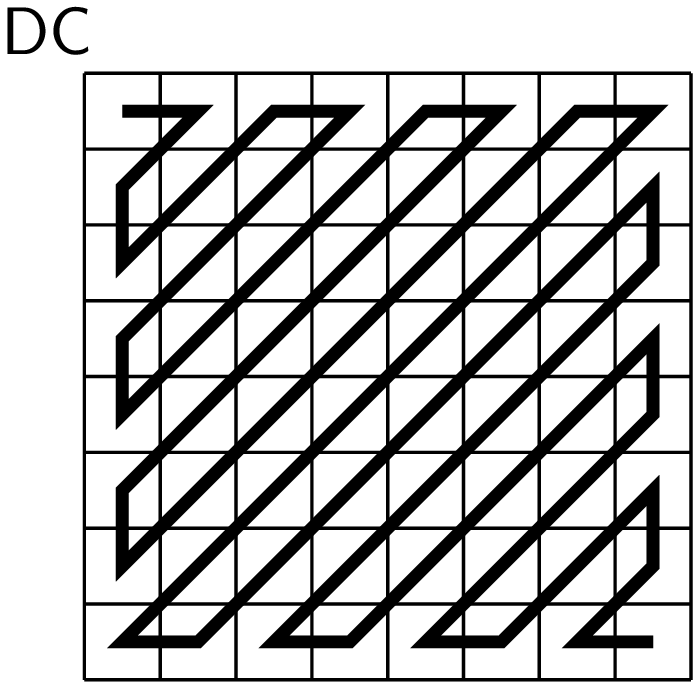
\includegraphics[width=3cm]{zigzag}
  \end{center}
  in order to (partially) sorter the coefficients attending to their
  magnitude. Notice that, after a given coefficient, the remainder
  ones are zero. This situation if encoded using the EOB (End Of
  Block) special symbol.
\item Encode the runs of non-zero coefficients using a variable-length
  code.\footnote{It is possible to use Huffman and arithmetic
    coding. However, the marginal gain of the last one (about a 10\%)
    and the patents that are behind it cause that the Huffman version
    is the most used one.}
\end{enumerate}

\section{Interlacing of the color components}
\begin{itemize}
\item Typically, in JPEG the 4:2:0 subsamplig pattern is the most used
  one (see Section \ref{sec:submuestreo}).
\item The color interlacing enables the pipelined (IO and CPU)
  reconstruction of the images row-by-row.
  \begin{enumerate}
  \item With interlacing:
    \begin{center}
      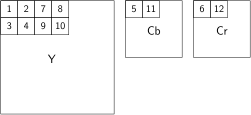
\includegraphics[width=8cm]{JPEG_entrelazamiento_componentes}
    \end{center}
    \newpage
  \item Without interlacing:
    \begin{center}
      %\texfigure{!}{!}{JPEG_no_entrelazamiento_componentes}
      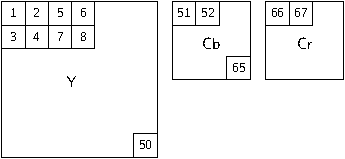
\includegraphics[width=8cm]{JPEG_no_entrelazamiento_componentes}
    \end{center}
  \end{enumerate}
\end{itemize}

\section*{Example}
\begin{itemize}
\item Let's encode a block of a grayscale image (luminance of
  ``lena'').
  \begin{center}
    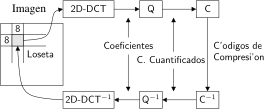
\includegraphics[width=8cm]{JPEG_codec}
  \end{center}
\end{itemize}

\newpage
\subsection*{$8\times 8$-DCT}
\begin{center}
  \resizebox{\textwidth}{!}{
    \begin{tabular}{ccc}
      \begin{tabular}{|rrrrrrrr|}
        \hline
        79 &75 &79 &82 &82 &86 &94 &94 \\
        76 &78 &76 &82 &83 &86 &85 &94 \\
        72 &75 &67 &78 &80 &78 &74 &82 \\
        74 &76 &75 &75 &86 &80 &81 &79 \\
        73 &70 &75 &67 &78 &78 &79 &85 \\
        69 &63 &68 &69 &75 &78 &82 &80 \\
        76 &76 &71 &71 &67 &79 &80 &83 \\
        72 &77 &78 &69 &75 &75 &78 &78 \\
        \hline
      \end{tabular}
      &
      $\Leftrightarrow$
      &
      \begin{tabular}{|rrrrrrrr|}
        \hline
        619 & -29 & 8 & 2 & 1 & -3 & 0 & 1\\
        22 & -6 & -4 & 0 & 7 & 0 & -2 & -3 \\
        11 & 0 & 5 & -4 & -3 & 4 & 0 & -3\\
        2 & -10 & 5 & 0 & 0 & 7 & 3 & 2\\
        6 & 2 & -1 & -1 & -2 & 0 & 0 & 8\\
        1 & 2 & 1 & 2 & 0 & 2 & -2 & -2\\
        -8 & -2 & -4 & 1 & 2 & 1 & -1 & 1\\
        -3  & 1 & 5 & -2 & 1 & -1 & 1 & -3\\
        \hline
      \end{tabular}
    \end{tabular}
  }
\end{center}
\begin{itemize}
\item Notice that the most part of the energy is concentrated in the
  DC coefficient and in the AC subrrounding coefficients.
\end{itemize}

\subsection*{Quantization}
\begin{center}
  \resizebox{\textwidth}{!}{
    \begin{tabular}{cccc}
      \begin{tabular}{|rrrrrrrr|}
        \hline
        619 & -29 & 8 & 2 & 1 & -3 & 0 & 1\\
        22 & -6 & -4 & 0 & 7 & 0 & -2 & -3 \\
        11 & 0 & 5 & -4 & -3 & 4 & 0 & -3\\
        2 & -10 & 5 & 0 & 0 & 7 & 3 & 2\\
        6 & 2 & -1 & -1 & -2 & 0 & 0 & 8\\
        1 & 2 & 1 & 2 & 0 & 2 & -2 & -2\\
        -8 & -2 & -4 & 1 & 2 & 1 & -1 & 1\\
        -3  & 1 & 5 & -2 & 1 & -1 & 1 & -3\\
        \hline
      \end{tabular}
      &
      div
      &
      \begin{tabular}{|rrrrrrrr|}
        \hline
        16 & 11 & 10 & 16 & 24 & 40 & 51 & 61 \\
        12 & 12 & 14 & 19 & 26 & 58 & 60 & 55 \\
        14 & 13 & 16 & 24 & 40 & 57 & 69 & 56 \\
        14 & 17 & 22 & 29 & 51 & 87 & 80 & 62 \\
        18 & 22 & 37 & 56 & 68 & 109 & 103 & 77 \\
        24 & 35 & 55 & 64 & 81 & 104 & 113 & 92 \\
        49 & 64 & 78 & 87 & 103 & 121 & 120 & 101 \\
        72 & 92 & 95 & 98 & 112 & 100 & 103 & 99 \\
        \hline
      \end{tabular}
      =\\
      &&&
    \end{tabular}
  }
  \begin{tabular}{|rrrrrrrr|}
    \hline
    39 & -3 & 1 & 0 & 0 & 0 & 0 & 0 \\
    2 & -1 & 0 & 0 & 0 & 0 & 0 & 0 \\
    1 & 0 & 0 & 0 & 0 & 0 & 0 & 0 \\
    0 & -1 & 0 & 0 & 0 & 0 & 0 & 0 \\
    0 & 0 & 0 & 0 & 0 & 0 & 0 & 0 \\
    0 & 0 & 0 & 0 & 0 & 0 & 0 & 0 \\
    0 & 0 & 0 & 0 & 0 & 0 & 0 & 0 \\
    0 & 0 & 0 & 0 & 0 & 0 & 0 & 0 \\
    \hline
  \end{tabular}
\end{center}
\begin{itemize}
\item Notice that the high frecuencies have been erased.
\end{itemize}

\subsection*{EOB generation}
\begin{itemize}
  \item The coeficients of the matrix
    \begin{center}
      \begin{tabular}{|rrrrrrrr|}
        \hline
        39 & -3 & 1 & 0 & 0 & 0 & 0 & 0 \\
        2 & -1 & 0 & 0 & 0 & 0 & 0 & 0 \\
        1 & 0 & 0 & 0 & 0 & 0 & 0 & 0 \\
        0 & -1 & 0 & 0 & 0 & 0 & 0 & 0 \\
        0 & 0 & 0 & 0 & 0 & 0 & 0 & 0 \\
        0 & 0 & 0 & 0 & 0 & 0 & 0 & 0 \\
        0 & 0 & 0 & 0 & 0 & 0 & 0 & 0 \\
        0 & 0 & 0 & 0 & 0 & 0 & 0 & 0 \\
        \hline
      \end{tabular}
    \end{center}
    are visited using the zig-zag scan to tind the EOB. The result is
  \begin{center}
    \begin{tabular}{ccccccccccccc}
      39 & -3 & 2 & 1 & -1 & 1 & 0 & 0 & 0 & 0 & 0 & -1 & EOB
    \end{tabular}
  \end{center}
\end{itemize}

\section{Entropy encoding of the runs}
\begin{itemize}
\item \textbf{Encoding of the DC coefficient.} Substract to the DC
  coefficient the previous one. In the last example, we have
  $39-34=5$. This value is encoded as a residue using the LS-JPEG
  encoding machinery (see Section
  \ref{sec:compresion_huffman_LS-JPEG}). The result is $100101_2$.
\item \textbf{Encoding of the AC coefficients.} We encode the pairs
  <number-of-previous-zeros,non-zero-value> in two steps.
  \begin{enumerate}
  \item Find the $SSSS$ category correspoding to the AC coefficient. For
    example, if the coefficient is $-3$, we determine that
    $SSSS\leftarrow 2$ (see Section
    \ref{sec:compresion_huffman_LS-JPEG}).
  \item Find the entry <number-of-previous-zeros,$SSSS$> in the table of
    AC codes proposed by the JPEG:
    \begin{center}
      \begin{tabular}{|r|r|l|}
        \multicolumn{3}{c}{JPEG AC codes (Luminance)}\\
        \hline
        Run/category & Longitud & Base code \\
        \hline
        0/0 & 4 & 1010 (=EOB) \\
        0/1 & 3 & 00 \\
        0/2 & 4 & 01 \\
        0/3 & 6 & 100 \\
        : & : & :\\
        15/10 & 26 & 1111 1111 1111 11110 \\
        \hline
      \end{tabular}
    \end{center}
    and output the base code bits. In our example, we output $01_2$.
  \item Execute the Step 3 of the LS-JPEG encoding algorithm taking $e=$
    the AC coeffient. In our example, we output $-3-2=-4$ using a binary
    number of $SSSS=2$ bits that is $00_2$.
  \end{enumerate}
\end{itemize}

The whole bit-stream for our example is:
\begin{center}
  \begin{tabular}{cccccccc}
    100101 & 0100 & 0110 & 001 & 000 & 001 & 11110100 & 1010
  \end{tabular}
\end{center}

Finally, the block is encoded using only $35$ bits. Therefore, the
compression ratio is 15:1 approximately ($0.55$ bits/pixel).

\section{Progressive transmission}
\begin{itemize}
\item Very useful when the images are transmited over slow links.
\item There are three positilities:
  \begin{enumerate}
  \item \textbf{Progressive transmission based on spectral selection:}
    \begin{itemize}
    \item All the low frequency coefficients are transmitted before
      than the rest of them.
    \item Provides up to 64 scans.
    \end{itemize}
  \item \textbf{Progressive transmission based on bit-plane selection:}
    \begin{itemize}
    \item The most significant bit-planes of all coefficients are
      transmitted before than the rest of them.
    \item Provides up to 11 scans.
    \end{itemize}
  \item \textbf{Progressive transmission based on a mixture of the
    last progressions:}
    \begin{itemize}
    \item 11 or even 64 scans could not be enough if the transmission
      time is big and the computational power of the received is
      high. In this case, the coefficients can be transmitted by
      bit-planes, but selecting also the coefficients attenting to
      their frequency.
    \item Up to 704 scans.
    \end{itemize}
  \end{enumerate}
\end{itemize}

\section{The hierarchical algorithm}
\begin{itemize}
\item It is based on building a differential pyramid and after that,
  every level of the pyramid (residue image) is compressed using the
  losy encoder or the lossless encoder.
\item To create the pyramid we can use the following algorithm:
  \begin{enumerate}
  \item Subsample (filtering previously) the image in a factor of 2 in
    each dimension.
  \item Interpolate the subsampled image in a factor of 2 in each
    dimension.
  \item Substract this image to the original one, obtaining a residue
    image that is the base of the pyramid (the high
    frequencies). Notice that if we add this image and the image
    obtained in the Step 1, we recover the original image.
  \item Repeat this process considering the subsampled image as the
    original one.
  \end{enumerate}
\item This multi-resolution representation is useful in those cases
  where the original resolution of the image is too large to the
  actual display/printing system.
\end{itemize}

\section{Motion JPEG (M-JPEG)}
\begin{itemize}
\item When each image of a sequece is compressed idependently using
  JPEG, we are using a Motion JPEG compressor.
\item Notice that, if the quality of the compression is constant, the size of each compressed image cound be different:
\end{itemize}
\begin{center}
  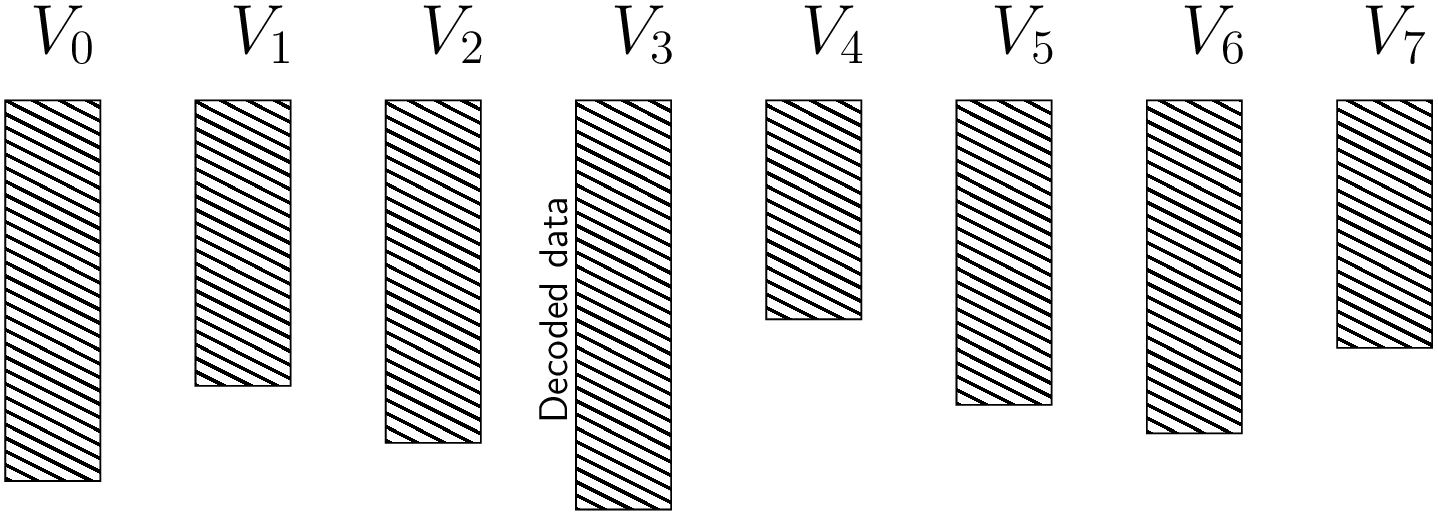
\includegraphics[width=0.7\textwidth]{M-JPEG_ir}
\end{center}

\section*{Lena $512\times 512$ RGB original}
\begin{center}
  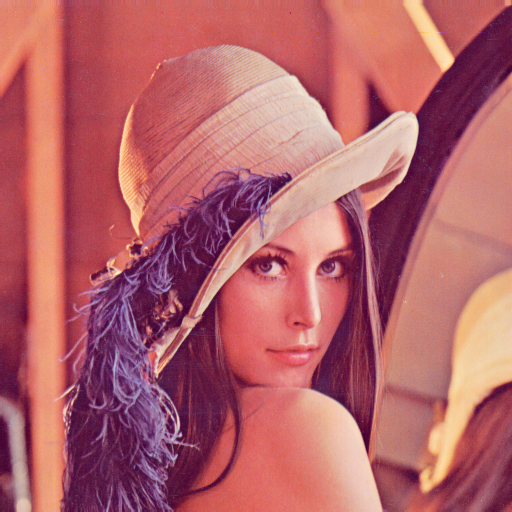
\includegraphics[height=7cm]{lena_rgb}
\end{center}

\section*{Lena at $1.0$ bpp ($\text{PSNR}=32.85$ dB)}
\begin{center}
  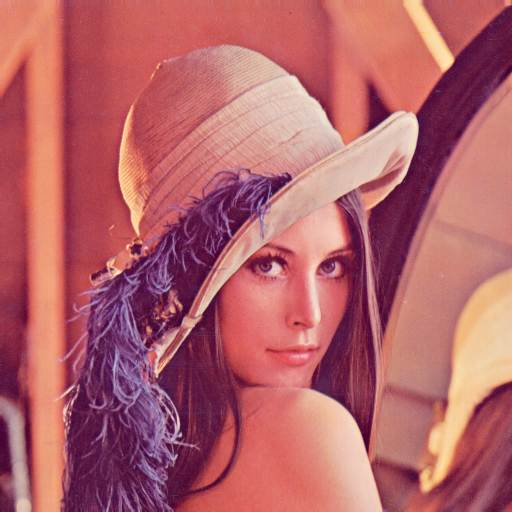
\includegraphics[height=7cm]{lena_10}
\end{center}

\section*{Lena at $0.5$ bpp ($\text{PSNR}=30.91$ dB)}
\begin{center}
  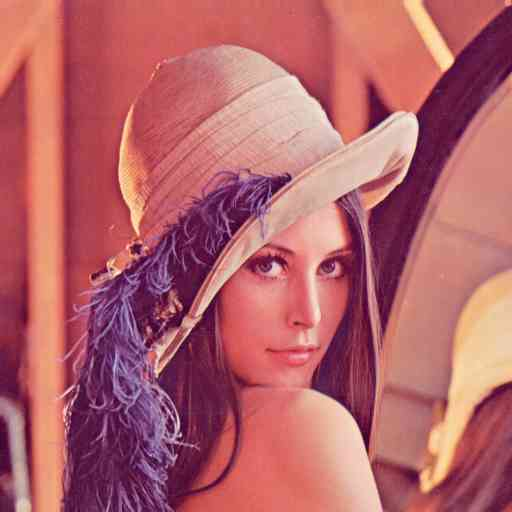
\includegraphics[height=7cm]{lena_05}
\end{center}

\section*{Lena at $0.4$ bpp ($\text{PSNR}=30.09$ dB)}
\begin{center}
  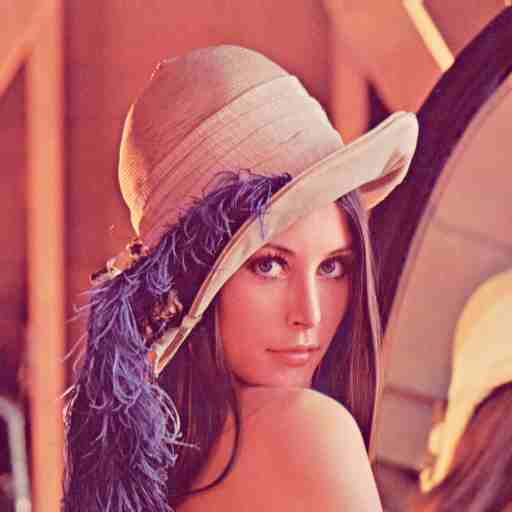
\includegraphics[height=7cm]{lena_04}
\end{center}

\section*{Lena at $0.3$ bpp ($\text{PSNR}=28.97$ dB)}
\begin{center}
  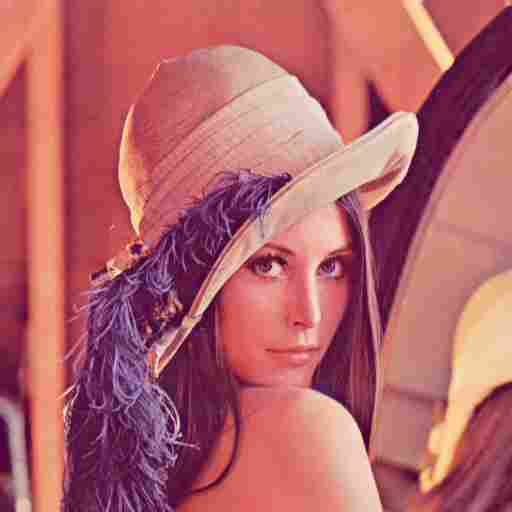
\includegraphics[height=7cm]{lena_03}
\end{center}

\section*{Lena at $0.2$ bpp ($\text{PSNR}=26.64$ dB)}
\begin{center}
  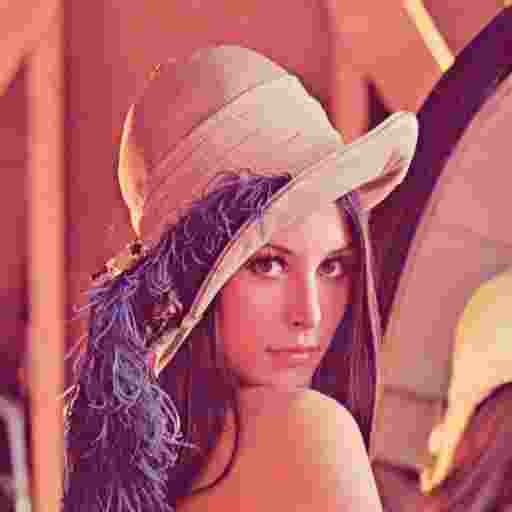
\includegraphics[height=7cm]{lena_02}
\end{center}

\section*{Lena at $0.1$ bpp ($\text{PSNR}=21.29$ dB)}
\begin{center}
  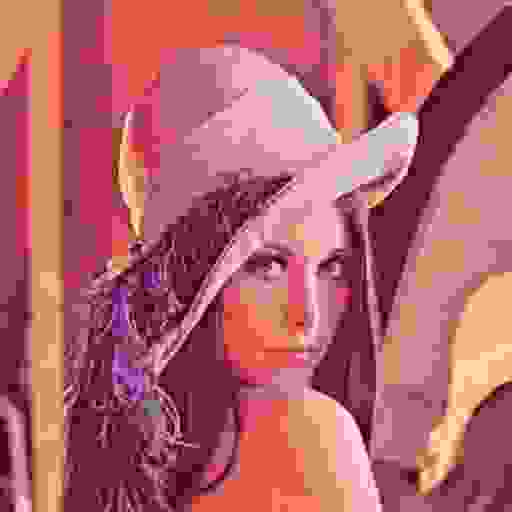
\includegraphics[height=7cm]{lena_01}
\end{center}

\section{Lab}
\begin{itemize}
\item Download and compile the
  \href{http://www.ace.ual.es/~vruiz/docencia/doctorado/snr.c}{\texttt{snr.c}}
  command line tool.
\item For each image of the
  \href{http://www.ace.ual.es/~vruiz/images/}{the Image Compression
    Corpus}, build a table with the structure:
\begin{verbatim}
# bpp MSE
\end{verbatim}
where the bpp (bit per pixel) is the result of compute the resulting
bit-rate after compress and decompress the images using the command
line tools \texttt{cjpeg} and \texttt{djpeg}.
\item Use \texttt{gnuplot} to draw the rate-distortion curve of JPEG
  for each of the test images.
\end{itemize}


\begin{comment}
\item En el Apéndice \ref{ape:vids_make} se presenta un fichero
  \texttt{Makefile} que muestra cómo invocar al programa
  \textit{FFMPEG} (\texttt{ffmpeg.mplayerhq.hu}) para generar una
  secuencia de vídeo en formato M-JPEG.
\item Acceda al directorio \texttt{vids} que encontrará a la misma
  altura que este documento en el sistema de ficheros y visualice los
  vídeos \texttt{*MJPEG*}.
\item En Linux se recomienda usar el programa \textit{MPlayer}
  (\texttt{www.mplayerhq.hu}). Para lanzarlo ejecutar, por ejemplo:
\begin{verbatim}
mplayer -loop 0 -fs archivo_video
\end{verbatim}
\item  Bajo Windows se recomienda usar el programa \textit{VLC media
    player} (\texttt{www.videolan.org}).
\end{comment}

\bibliographystyle{plain}
\bibliography{JPEG,image-standards}
